\section{Recherche de documents}
\label{sec:recherche}

La plateforme joue en quelque sorte le rôle d'un moteur de recherche. L'idée est de fournir aux utilisateurs une recherche riche et diverse qui lui permettra de trouver efficacement des journaux, des articles ou des revues de presse qu'il souhaiterait consulter. On veut donc permettre à l'utilisateur d'effectuer trois types de recherches; suivant le type des documents qu'il recherche. Cette fonctionnalité est une fonctionnalité importante pour l'utilisateur, l'enjeu étant de lui permettre de trouver le plus efficacement possible des documents qui peuvent l'intéresser.

Nous avons décidé qu'un utilisateur ne pourra pas chercher en même temps des 'articles' et des 'journaux' pour distinguer ces différents types et d'éviter de rendre trop de résultats inintéressants. Suivant le type de document recherché l'utilisateur disposera de plusieurs filtres qui seront mis à jour sur la page ; ces filtres dépendront bien évidemment du type de document sélectionné.

Il sera bien évidemment possible de trier les résultats par date ; par ordre chronologique de parution ou non.

\subsection{Recherche de journaux}
\label{sec:recherche_journal}

La première recherche élémentaire est celle des journaux. L'utilisateur, en arrivant sur cette page, devra être capable de pouvoir chercher l'édition d'un journal qui l'intéresse. Pour ça, il pourra effectuer une recherche sur le nom de celui-ci, mais aussi sur la date. Si le nombre de journaux différents n'est pas trop important, l'utilisateur disposera directement d'une liste de tous les journaux. Pour la date, il aura le choix de la filtrer suivant trois catégories : 'AVANT', lui permettant de trouver toutes les éditions sorties avant une certaine date, 'APRES', permettant au contraire d'obtenir les éditions sorties après la date écrite. Enfin 'ENTRE' permettra de chercher des journaux édités entre deux dates précises. Pour rechercher sur une date, l'utilisateur devra au minimum rentrer l'année et pourra jusqu'à rentrer le jour et le mois. Il sera bien évidemment possible de chercher plusieurs journaux. Un utilisateur pourra chercher des éditions de 1940 de 'Libération' et du 'Canard enchaîné' en même temps ; il suffira de sélectionner ces deux-là dans la liste de journaux avant de lancer la recherche.

Les résultats affichés donneront le nom du journal et sa date de parution. Cliquer sur un des résultats permettra d'arriver sur la page de consultation de document pour lire ce dernier.

En résumé, la recherche de journaux s'effectuera sur deux attributs :
\begin{itemize}
	\item Le nom du journal
	\item La date d'édition
\end{itemize}

\subsection{Recherche d'articles}
\label{sec:recherche_article}

La seconde recherche essentielle de la plateforme sera la recherche d'articles. Habituellement un utilisateur lisant un journal se retrouvera assez souvent à chercher des informations sur des évènements particuliers qui auraient pu se dérouler. Dans ce but, ou dans le cas où un utilisateur souhaiterait créer une revue de presse d'articles spécifiques, il est nécessaire de permettre à l'utilisateur de pouvoir chercher avec de nombreux filtres différents des articles.

Les deux premiers filtres sont les mêmes que pour les journaux et suivent le même fonctionnement; l'utilisateur pourra chercher des articles d'un (ou de plusieurs) journal spécifique et suivant une date spécifique. Un autre filtre essentiel pour cette recherche est bien évidemment la recherche sur un titre d'article. L'utilisateur aura un champ qui recherchera donc spécifiquement sur le titre des articles stockés. L'utilisateur pourra aussi effectuer une recherche sur le contenu de l'article. À l'instar d'une recherche google, il sera possible de rentrer du texte qui sera cherché dans le texte d'un article; et les occurrences des mots recherchés seront mis en évidence (gras) dans le résultat de recherche. Un autre élément de recherche, plus spécifique, mais qui peut rester utile (dans le cadre d'une revue de presse sur une personne), est la recherche sur l'auteur d'un article. Un champ sera disponible pour chercher des articles écrits par une certaine personne. Enfin, il sera possible pour l'utilisateur de chercher des articles suivant les tags qui lui ont été associés. À la manière de twitter, une auto-complétion lui permettra de rentrer des tags qui ont été définis auparavant, cela lui permettra d'être sûr de ne pas rentrer des tags qui n'existeraient pas.

Les résultats affichés contiendront le nom de l'article, le nom du journal d'appartenance, la date de parution, l'auteur, la liste des tags associés à celui-ci et quelques lignes de début de l'article. Si une recherche dans le contenu de l'article était effectuée, alors à la place les lignes affichées présenterons le contexte dans lequel les mots ont été trouvés. Cliquer sur un résultat amènera l'utilisateur sur la visionneuse de document avec l'article pré-sélectionné.

Il sera par ailleurs possible de trier ces articles en deux catégories; les articles appartenant à une revue de presse et les autres. Les résultats d'articles appartenant à une revue de presse auront un fond coloré, permettant de les identifier.

En résumé, la recherche d'articles s'effectuera sur six attributs :
\begin{itemize}
	\item le journal dans lequel il est paru;
	\item la date de parution;
	\item le titre de l'article;
	\item les tags associés à l'article;
	\item le contenu de l'article;
	\item l'auteur de l'article.
\end{itemize}

\subsection{Recherche de revues de presse}
\label{sec:recherche_revue}

Le dernier type de recherche disponible pour l'utilisateur se trouve être la recherche sur les revues de presse. Cela lui permettra de ne pas avoir à chercher dans la liste des revues de presse une revue qui l'intéresse. Cette recherche est assez simple; l'utilisateur pourra effectuer une recherche sur le nom de la revue de presse et sur la description de celle-ci.

Les résultats affichés contiendront le nom de la revue de presse, sa description et les trois premiers articles de celle-ci. Cliquer sur un résultat amènera l'utilisateur sur la page de la revue de presse. Il sera par ailleurs possible de trier les résultats obtenus suivant la date de création de la revue de presse, mais aussi la date de la dernière modification de celle-ci.

En résumé, la recherche de revues de presse s'effectuera sur deux attributs :
\begin{itemize}
	\item Le nom de la revue de presse
	\item La description de la revue de presse
\end{itemize}
\bigskip
\par
D'après les spécifications pour la fonctionnalité de recherche; on arrive à un croquis de la page rassemblant toutes ces fonctionnalités qui devrait prendre la forme suivante. (Figure \ref{fig:recherche_img})

    \begin{figure}[H]
        \centering
        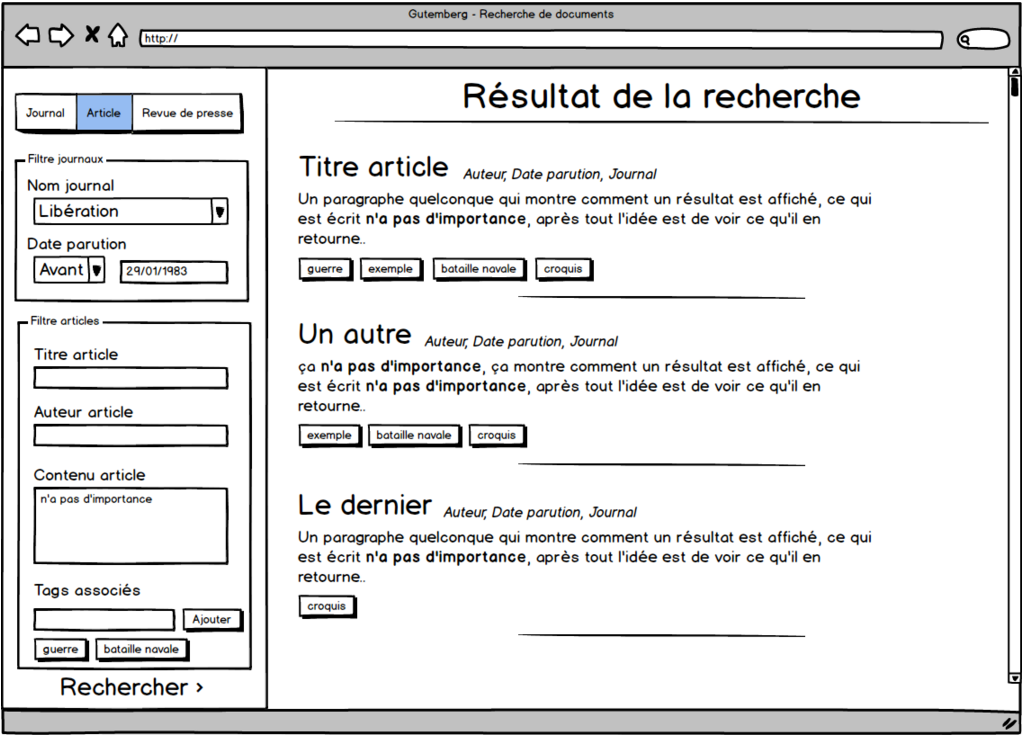
\includegraphics[width=\textwidth]{figures/recherche.png}
            \caption{Page de recherche d'un article}
            \label{fig:recherche_img}
    \end{figure}